\documentclass{article}
\usepackage{hyperref}
\usepackage {graphicx, amsmath}
\usepackage[margin=1.0in]{geometry}
\title{F24 CSE220 Lab2}
\author{
  Andrew Bruce \\ \href{mailto:acbruce@ucsc.edu}{acbruce@ucsc.edu} \and
  Mohit Agrawal \\ \href{mailto:mmagrawa@ucsc.edu}{mmagrawa@ucsc.edu}
}

\begin{document}
\maketitle

\section*{Part1}
\subsection*{IPC}
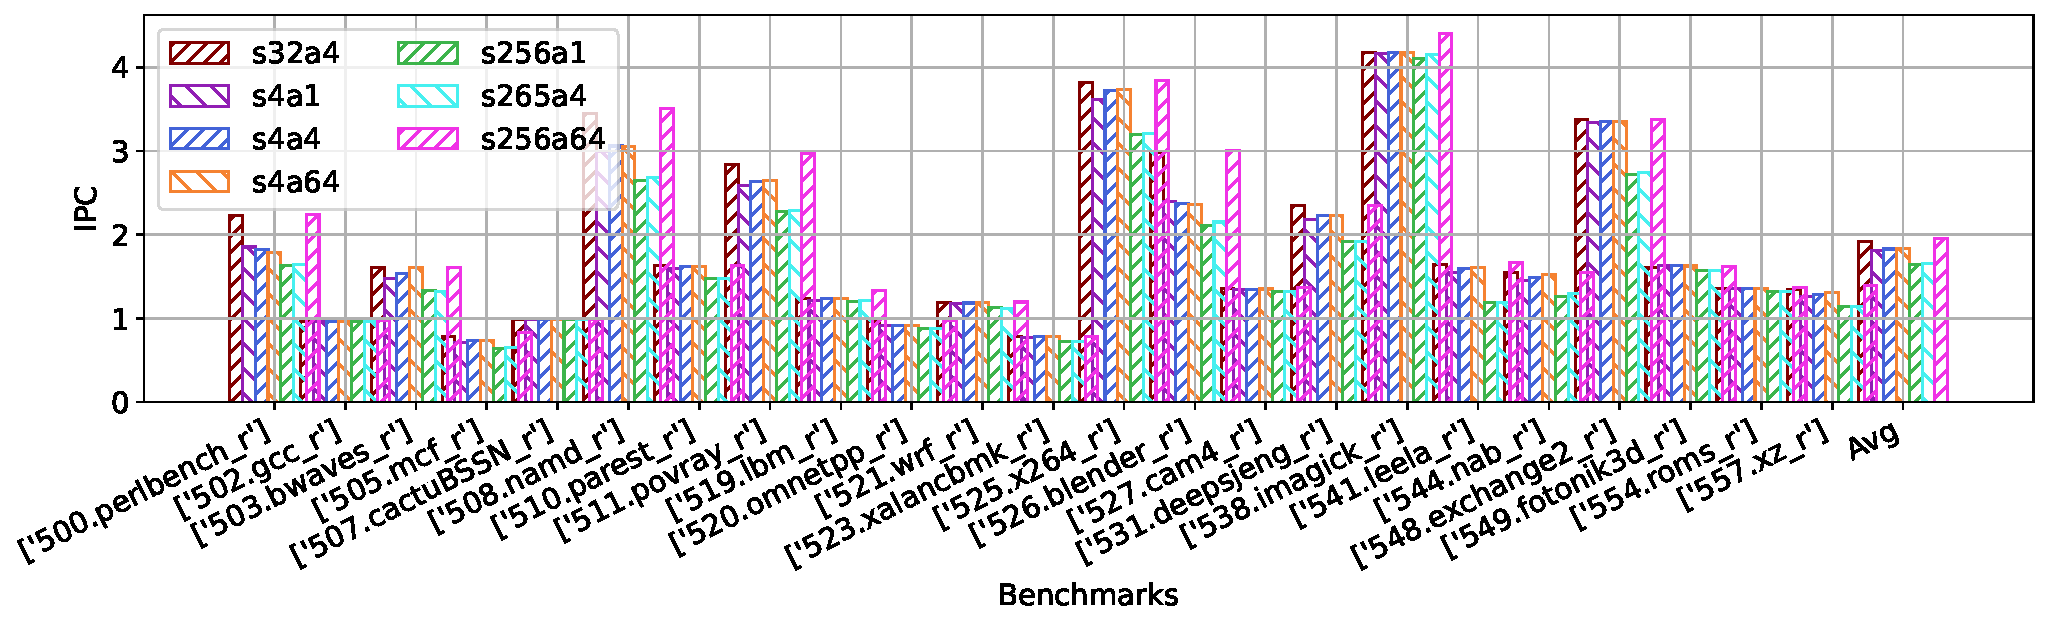
\includegraphics[width=\textwidth]{Part1/IPC.pdf}.
In this plot increasing both the size and assosiativity of the cache increases the IPC for almost every single test. Increasing the associativity from 1 to 4 was not as effective as increasing the size from 4kb to 256kb at increasing IPC.
\subsection*{DCache miss rate}
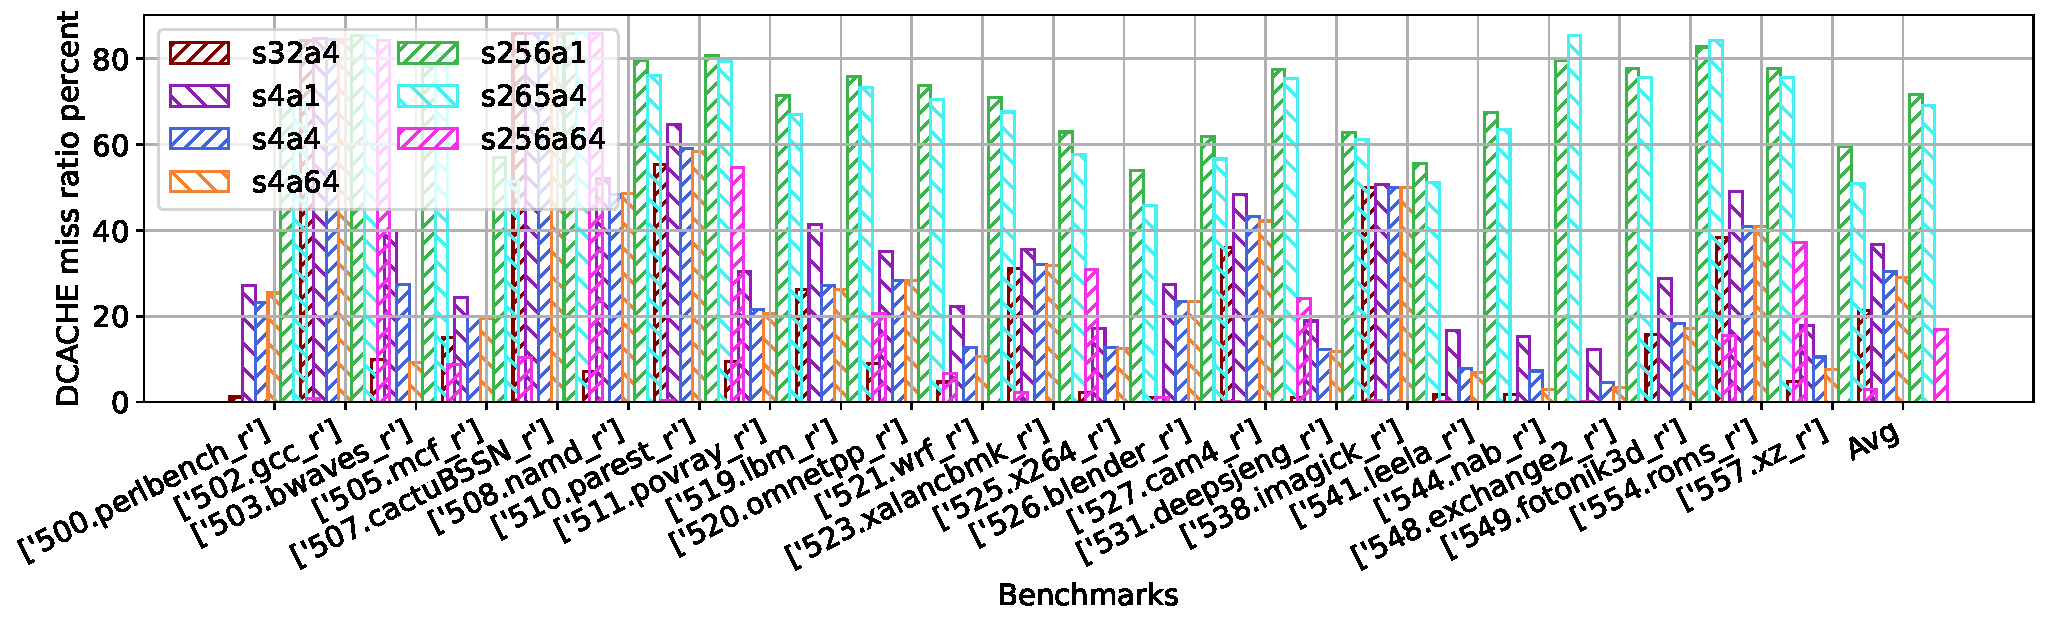
\includegraphics[width=\textwidth]{Part1/DCACHE.pdf}.
Outside of GCC and cactuBSSN, increasing the cache size to 256 kb universally decreased the miss ratio of the dcache. Increasing assosiativity also lowered the miss ratio. We also notice that the size 32 configuration performed surprisingly well compared to the 264 configurations showing the ability to get similar performance with less complexity by having a good associativity to capacity ratio. 
\section*{Part3}
\subsection*{DCache miss types}
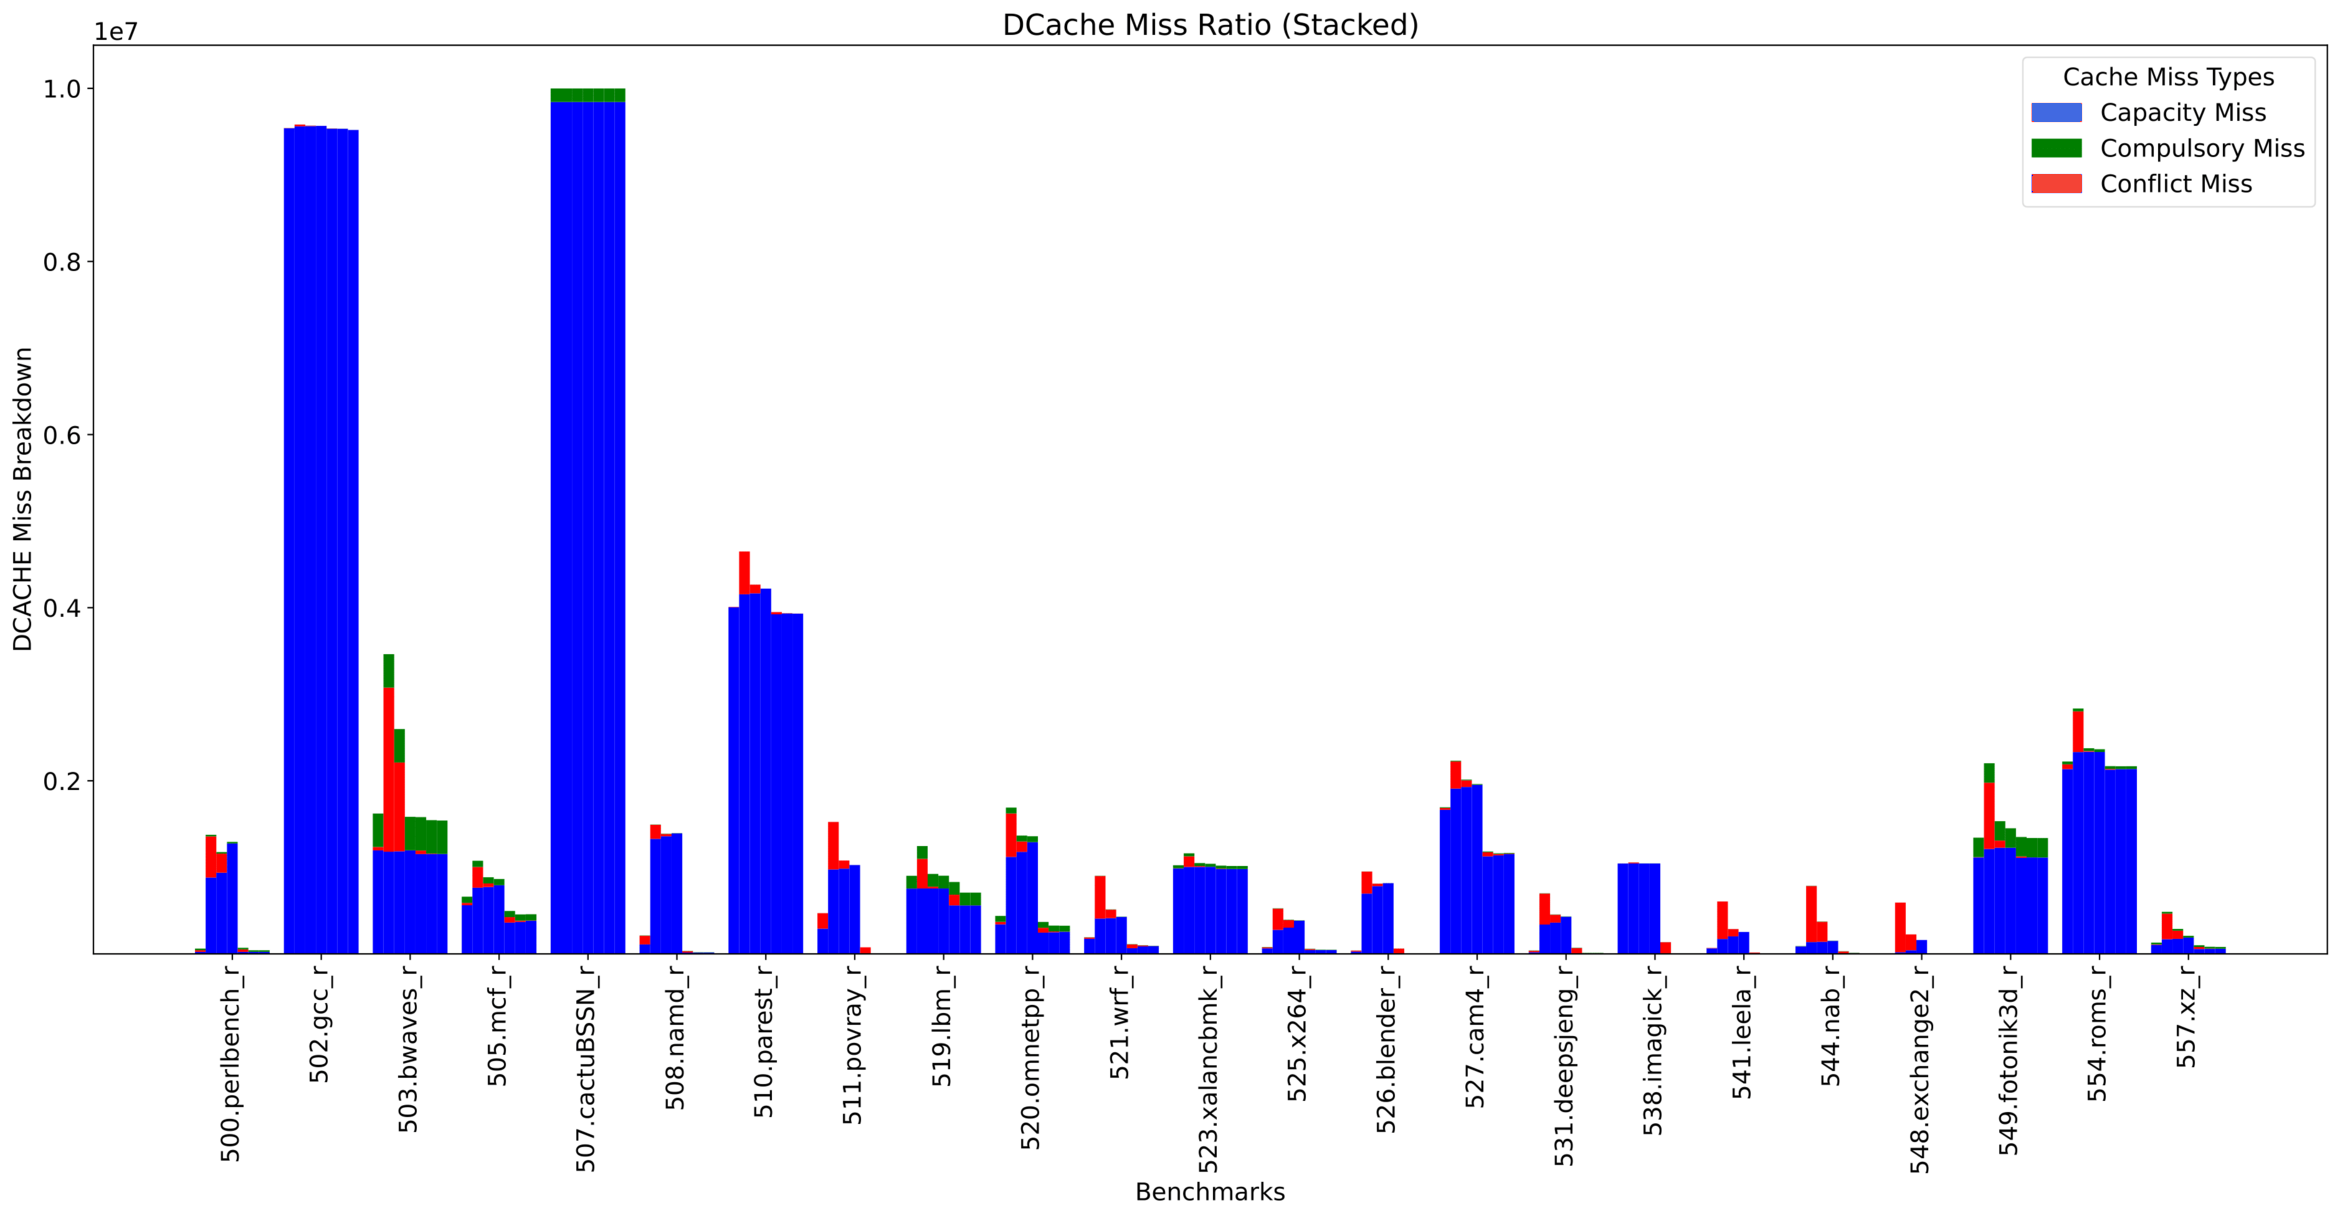
\includegraphics[width=\textwidth]{Part3_4/DCACHE_MISS_STACKED.png}.
This graph is the same as the dcache miss rate but with stacked bars to show the cache miss type. \\

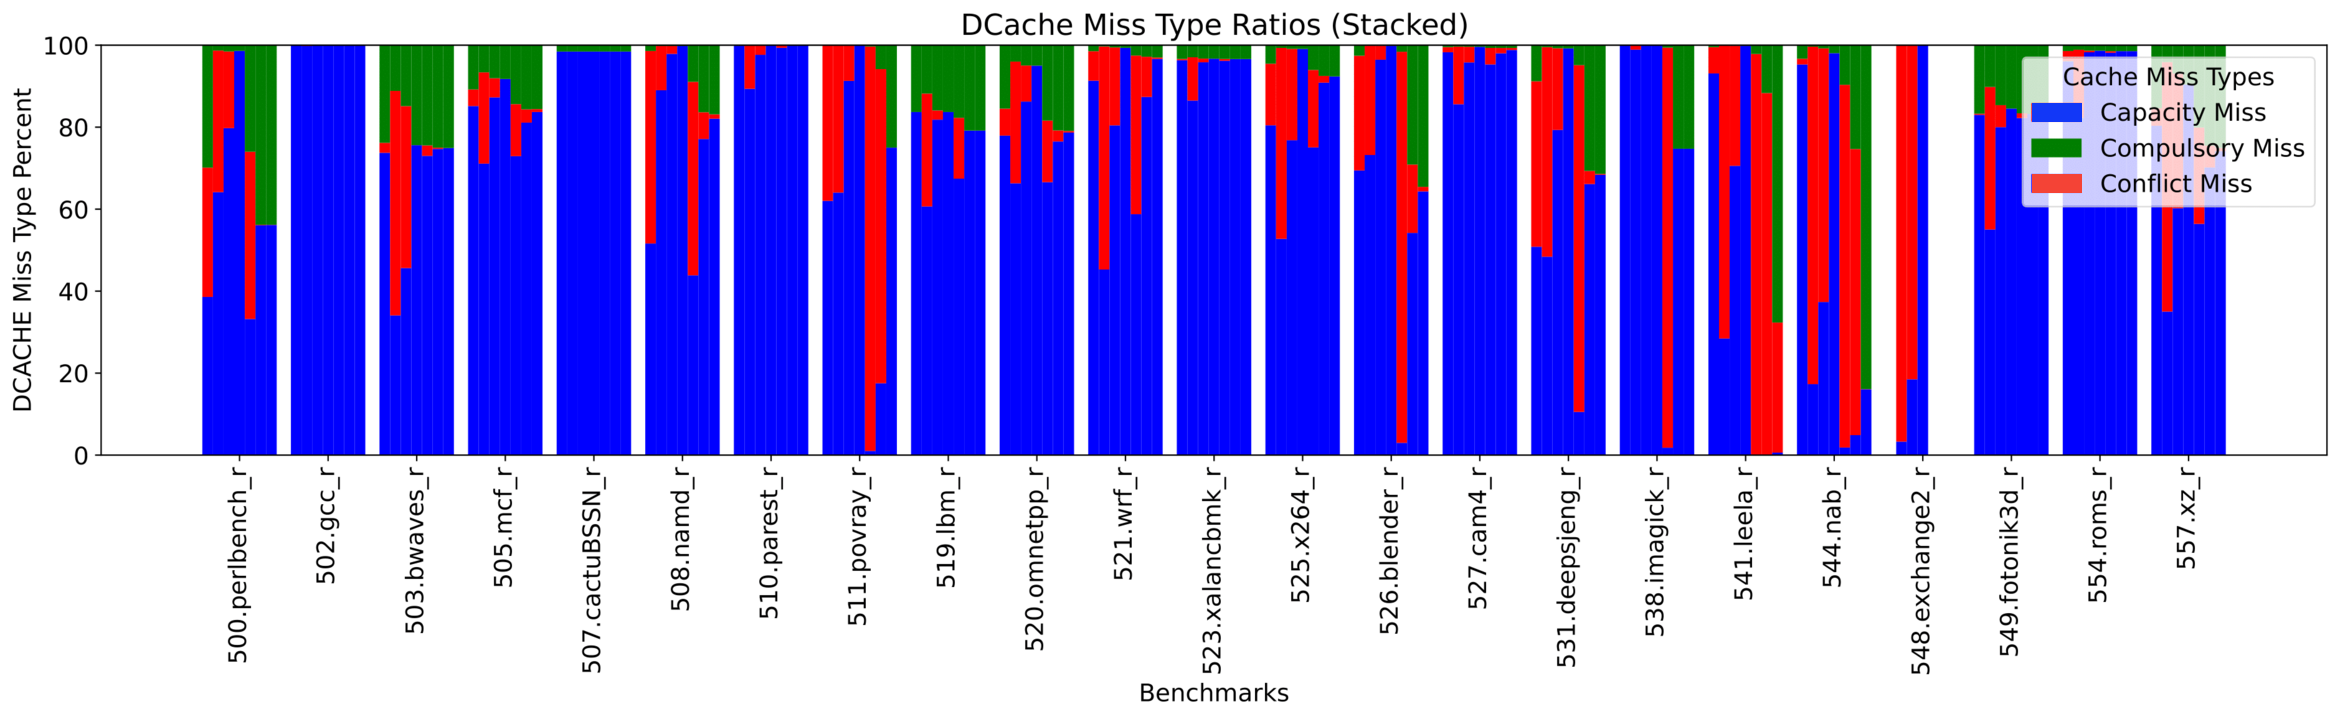
\includegraphics[width=\textwidth]{Part3_4/DCACHE_MISS_STACKED_RATIO.png}.
This graph shows the ratio of the types of misses for each configuration. \\

Overall we notice that the vast majority of misses are capacity misses with compulsory misses being the least common, possibly because they only happen once per block. We notice that the Capacity misses for the configurations with the same size is roughly the same due to capacity misses primarily being due to how limited the size of the cache is. The Conflict misses are more affected by the associativity as we can see between the s4a1 and s4a4 we notice a bigger red bar for s4a1, showing that a lower associativity can lead to more data fighting to be in the same spot. We believe that to improve our cache more it would be beneficial to increase the cache size more and also scale the associativity a little bit with it seeing as most of our misses are caused by Capacity misses and we notice a significant decrease in those misses once the size is increased and almost no conflict misses when our associativity is scaled well with the size of the cache. \\
\end{document}

